\documentclass[11pt]{article}
\usepackage{amsfonts,amsmath,latexsym,enumitem,amsthm,amsbsy}
\usepackage{xcolor}
\usepackage{tikz}
\usetikzlibrary{fit,shapes, arrows.meta,bending}
\usetikzlibrary{decorations.pathreplacing}

\begin{document}

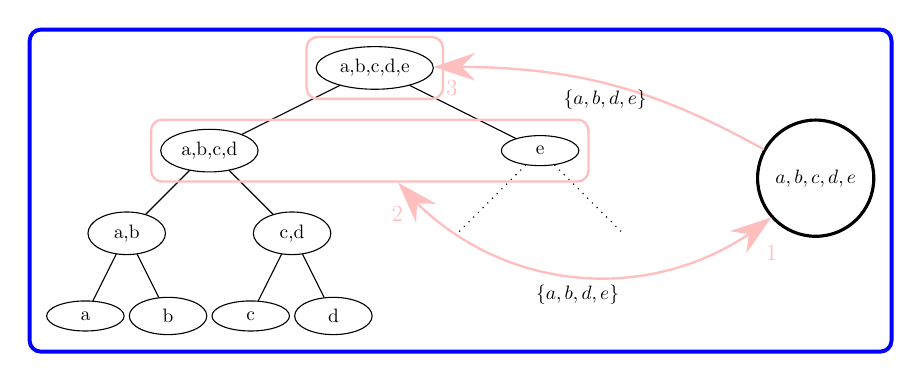
\begin{tikzpicture}[
    scale=0.7, transform shape,
    level 1/.style={sibling distance=60mm},
    level 2/.style={sibling distance=30mm},
    level 3/.style={sibling distance=15mm},
    ball/.style={draw, ellipse, minimum width=40pt},
    main_ball/.style={draw, circle, minimum width=60pt, line width=0.4mm},
    edge from parent/.style={draw},
    ball_e/.style={white, ellipse, minimum width=40pt},
]
\node[ball] (root) {a,b,c,d,e}
    child {
        node[ball] (abcd) {a,b,c,d}
        child {
            node[ball] {a,b}
            child { node[ball] (a) {a} }
            child { node[ball] (b) {b} }
        }
        child {
            node[ball] {c,d}
            child { node[ball] {c} }
            child { node[ball] {d} }
        }
    }
    child {
        node (x) [ball] {e}
    };
\draw[dotted] (x) -- ++(-1.5,-1.5);
\draw[dotted] (x) -- ++(1.5,-1.5);

\node (main) at (8, -2.0) [main_ball, label={[xshift=-0.8cm, yshift=-2.7cm, font=\large]$\textcolor{pink}{1}$}] {$a,b,c,d,e$}; 

\node[draw=pink, rounded corners, line width=0.3mm, fit=(abcd)(x), label={[xshift=0.5cm, yshift=-2.0cm, font=\large]$\textcolor{pink}{2}$}] (lower) {};

\node[draw=pink, rounded corners, line width=0.3mm, fit=(root), label={[xshift=1.4cm, yshift=-1.2cm, font=\large]$\textcolor{pink}{3}$}] (upper) {};

\draw[draw=pink, fill=pink, {Stealth[length=15pt,width=10pt]}-{Stealth[length=15pt,width=10pt]}] (lower) edge [line width=0.3mm, bend right=45] node[midway,below] {$\{a,b,d,e\}$}  (main);

\draw[draw=pink, fill=pink, -{Stealth[length=15pt,width=10pt]}] (main) edge [line width=0.3mm, bend right=15] node[midway,below] {$\{a,b,d,e\}$}  (root);

\node[inner sep=6pt, draw=blue, rounded corners, line width=0.5mm, fit=(x) (a)(b)(root)(main), ] {};
\end{tikzpicture}

\end{document}